\documentclass{article}
\usepackage[utf8]{inputenc}
\usepackage[spanish]{babel}
\usepackage[top=2cm, bottom=2cm, left=2.5cm, right=2.5cm]{geometry}

\usepackage{listings, listings-rust}
\usepackage{graphicx}
\graphicspath{{figures/}{../mockups/}}
\usepackage{caption}
\usepackage{enumitem}
\usepackage{dirtree}
\usepackage{hyperref}
\usepackage{xcolor}

\definecolor{codegreen}{rgb}{0,0.6,0}
\definecolor{codegray}{rgb}{0.5,0.5,0.5}
\definecolor{codepurple}{rgb}{0.58,0,0.82}
\definecolor{backcolour}{rgb}{0.95,0.95,0.92}

\lstdefinestyle{mystyle}{
    backgroundcolor=\color{backcolour},   
    commentstyle=\color{codegreen},
    keywordstyle=\color{magenta},
    numberstyle=\tiny\color{codegray},
    stringstyle=\color{codepurple},
    basicstyle=\ttfamily\footnotesize,
    breakatwhitespace=false,         
    breaklines=true,                 
    captionpos=b,                    
    keepspaces=true,                 
    numbers=left,                    
    numbersep=5pt,                  
    showspaces=false,                
    showstringspaces=false,
    showtabs=false,                  
    tabsize=2
}

\lstset{style=mystyle}

\title{Chat Multicliente}
\author{Evan Miranda}
\date{\today}

\begin{document}

% TODO: Hacer una portada

\begin{titlepage}
\centering
{\bfseries\LARGE Universidad Nacional Autónoma de México \par}
\vspace{1cm}
{\scshape\Large Facultad de Ciencias \par}
\vspace{3cm}
{\scshape\Huge Chat Multicliente \par}
\vspace{3cm}
{\itshape\Large Primer proyecto de Modelado y Programación \par}
\vfill
{\Large Autor: \par}
{\Large Evan Miranda Martínez \par}
\vfill
{\Large Septiembre 2026 \par}
\end{titlepage}

 \section{Resumen}

Este trabajo presenta \textbf{Gabby}, un sistema de chat multicliente con arquitectura
cliente-servidor, desarrollado como primer proyecto de la materia \textbf{Modelado y
Programación} de la licenciatura en \textbf{Ciencias de la Computación} de la
\textbf{Facultad de Ciencias, UNAM}. El documento aborda tanto el modelado del sistema como
su implementación: un cliente escrito en \textbf{Go}, con una interfaz de terminal construida
con la popular biblioteca \textbf{Bubble Tea} bajo la \textbf{Arquitectura Elm}, y un servidor escrito
en \textbf{Rust} y \textbf{Tokio}, sometido a pruebas de carga con 3,000 usuarios simultáneos.
 \section{Introducción}

\subsection*{Objetivo}
El objetivo general de este proyecto es diseñar e implementar un sistema de 
\textbf{Chat Multicliente} basado en la arquitectura cliente-servidor, que permita
la comunición en tiempo real entre múltiples clientes.

\subsection*{Alcance}

El alcance de este proyecto está delimitado en gran parte por el protocolo
establecido en clase. En términos funcionales, se trata de un chat
convencional con soporte para \textbf{mensajes públicos}, \textbf{salas} y
\textbf{mensajes privados}. No obstante, el alcance de \textbf{Gabby} se
amplió más allá de lo requerido, incorporando además una interfaz de
usuario moderna por terminal, pensando en mejorar la experiencia de usuario.


Sin embargo, \textbf{Gabby} sigue siendo bastante limitado en comparación a muchisimas 
de las alternativas disponibles. Especialmente debido a que no contiene, \textbf{cifrado}, 
\textbf{persistencia de datos}, \textbf{sistema de autentificación}, o \textbf{envío de archivos multimedia}.
 \section{Análisis y Diseño}

El \textbf{Chat Multicliente} puede dividirse fundamentalmente en dos programas independientes:
\textbf{cliente} y \textbf{servidor}. La comunicación entre ambas partes se realiza con \textbf{JSON}
sobre \textbf{TCP} por medio del protocolo establecido en el curso. El protocolo cuenta con \textbf{23}
mensajes establecidos, más un mensaje genérico de respuesta por parte del servidor.

\subsection*{Cliente}

El cliente se diseñó para ser desarrollado en el lenguaje de programación \textbf{Golang}, utilizando 
la biblioteca \textbf{Bubble Tea} para la interfaz de terminal. Esta decisión se tomó de manera previa
al análisis de la especificación del proyecto, pues estaba realmente entusiasmado en utilizar la 
biblioteca para algún proyecto. En consecuencia, \textbf{Gabby} adopta la \textbf{Arquitectura ELM}(\textit{Model-Update-View})
como arquitectura principal. 

La \textbf{Arquitectura ELM} surge en la comunidad del lenguaje de programación funcional \textbf{ELM}
como una manera de estructurar interfaces gráficas reactivas y funcionales. Se compone de estos tres elementos:

\begin{description}[leftmargin=2.2cm, style=nextline, font=\bfseries]
    \item[Modelo] Representa el estado actual de la aplicación.
    \item[Update] Ciclo que actualiza el Modelo a partir de mensajes recibidos.
    \item[Vista] Una fotografía del estado en un momento dado.
\end{description}

La arquitectura mantiene un flujo de datos unidireccional: \textbf{Modelo} $\Rightarrow$ \textbf{Update} $\Rightarrow$ 
\textbf{Vista}  $\Rightarrow$ \textbf{Modelo}. Y permite la comunicación entre componentes y etapas gracias a dos abstracciones: 
los \textbf{mensajes}, tipos de datos que notifican la ocurrencia de eventos, y los \textbf{comandos}, indicaciones para 
ejecutar acciones con efectos secundarios.

Generalmente, las aplicaciones realizadas a partir de la \textbf{Arquitectura ELM} cuentan con un modelo 
raíz que encapsula varios submodelos. Cada submodelo se encarga de la lógica de una parte específica y
delimitada de la interfaz manteniendo su propio estado, su propia función de actualización y su propia vista. 
El modelo raíz orquesta estos submodelos: delega los mensajes correspondientes a cada uno, integra sus vistas parciales 
en la vista general de la aplicación, y coordina la comunicación entre ellos cuando es necesario.

\begin{figure}[h]
    \centering
    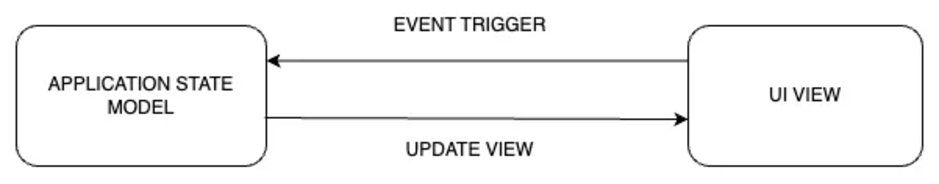
\includegraphics[width=0.6\textwidth]{flow.pdf}
    \caption{Flujo de datos de la arquitectura ELM}
    \label{fig:elm-flow} 
\end{figure}

\subsubsection*{Interfaz}

La interfaz de \textbf{Gabby} está fuertemente inspirada en interfaces de terminal populares, como \textbf{Lazygit} y \textbf{Lazydocker}. 
Por lo tanto, tanto la experiencia de usuario como el diseño visual retoman los recursos característicos de esta filosofía, es decir: 
distribución de la información en paneles, formularios modales para la captura de datos, y una navegación por atajos de teclado modal y 
basada en aspectos mnemotécnicos.

Esto es bastante visible en la figura \ref{fig:mockup-cliente}. En ella podemos observar varias de las características antes mencionadas.

\begin{figure}[h]
    \centering
    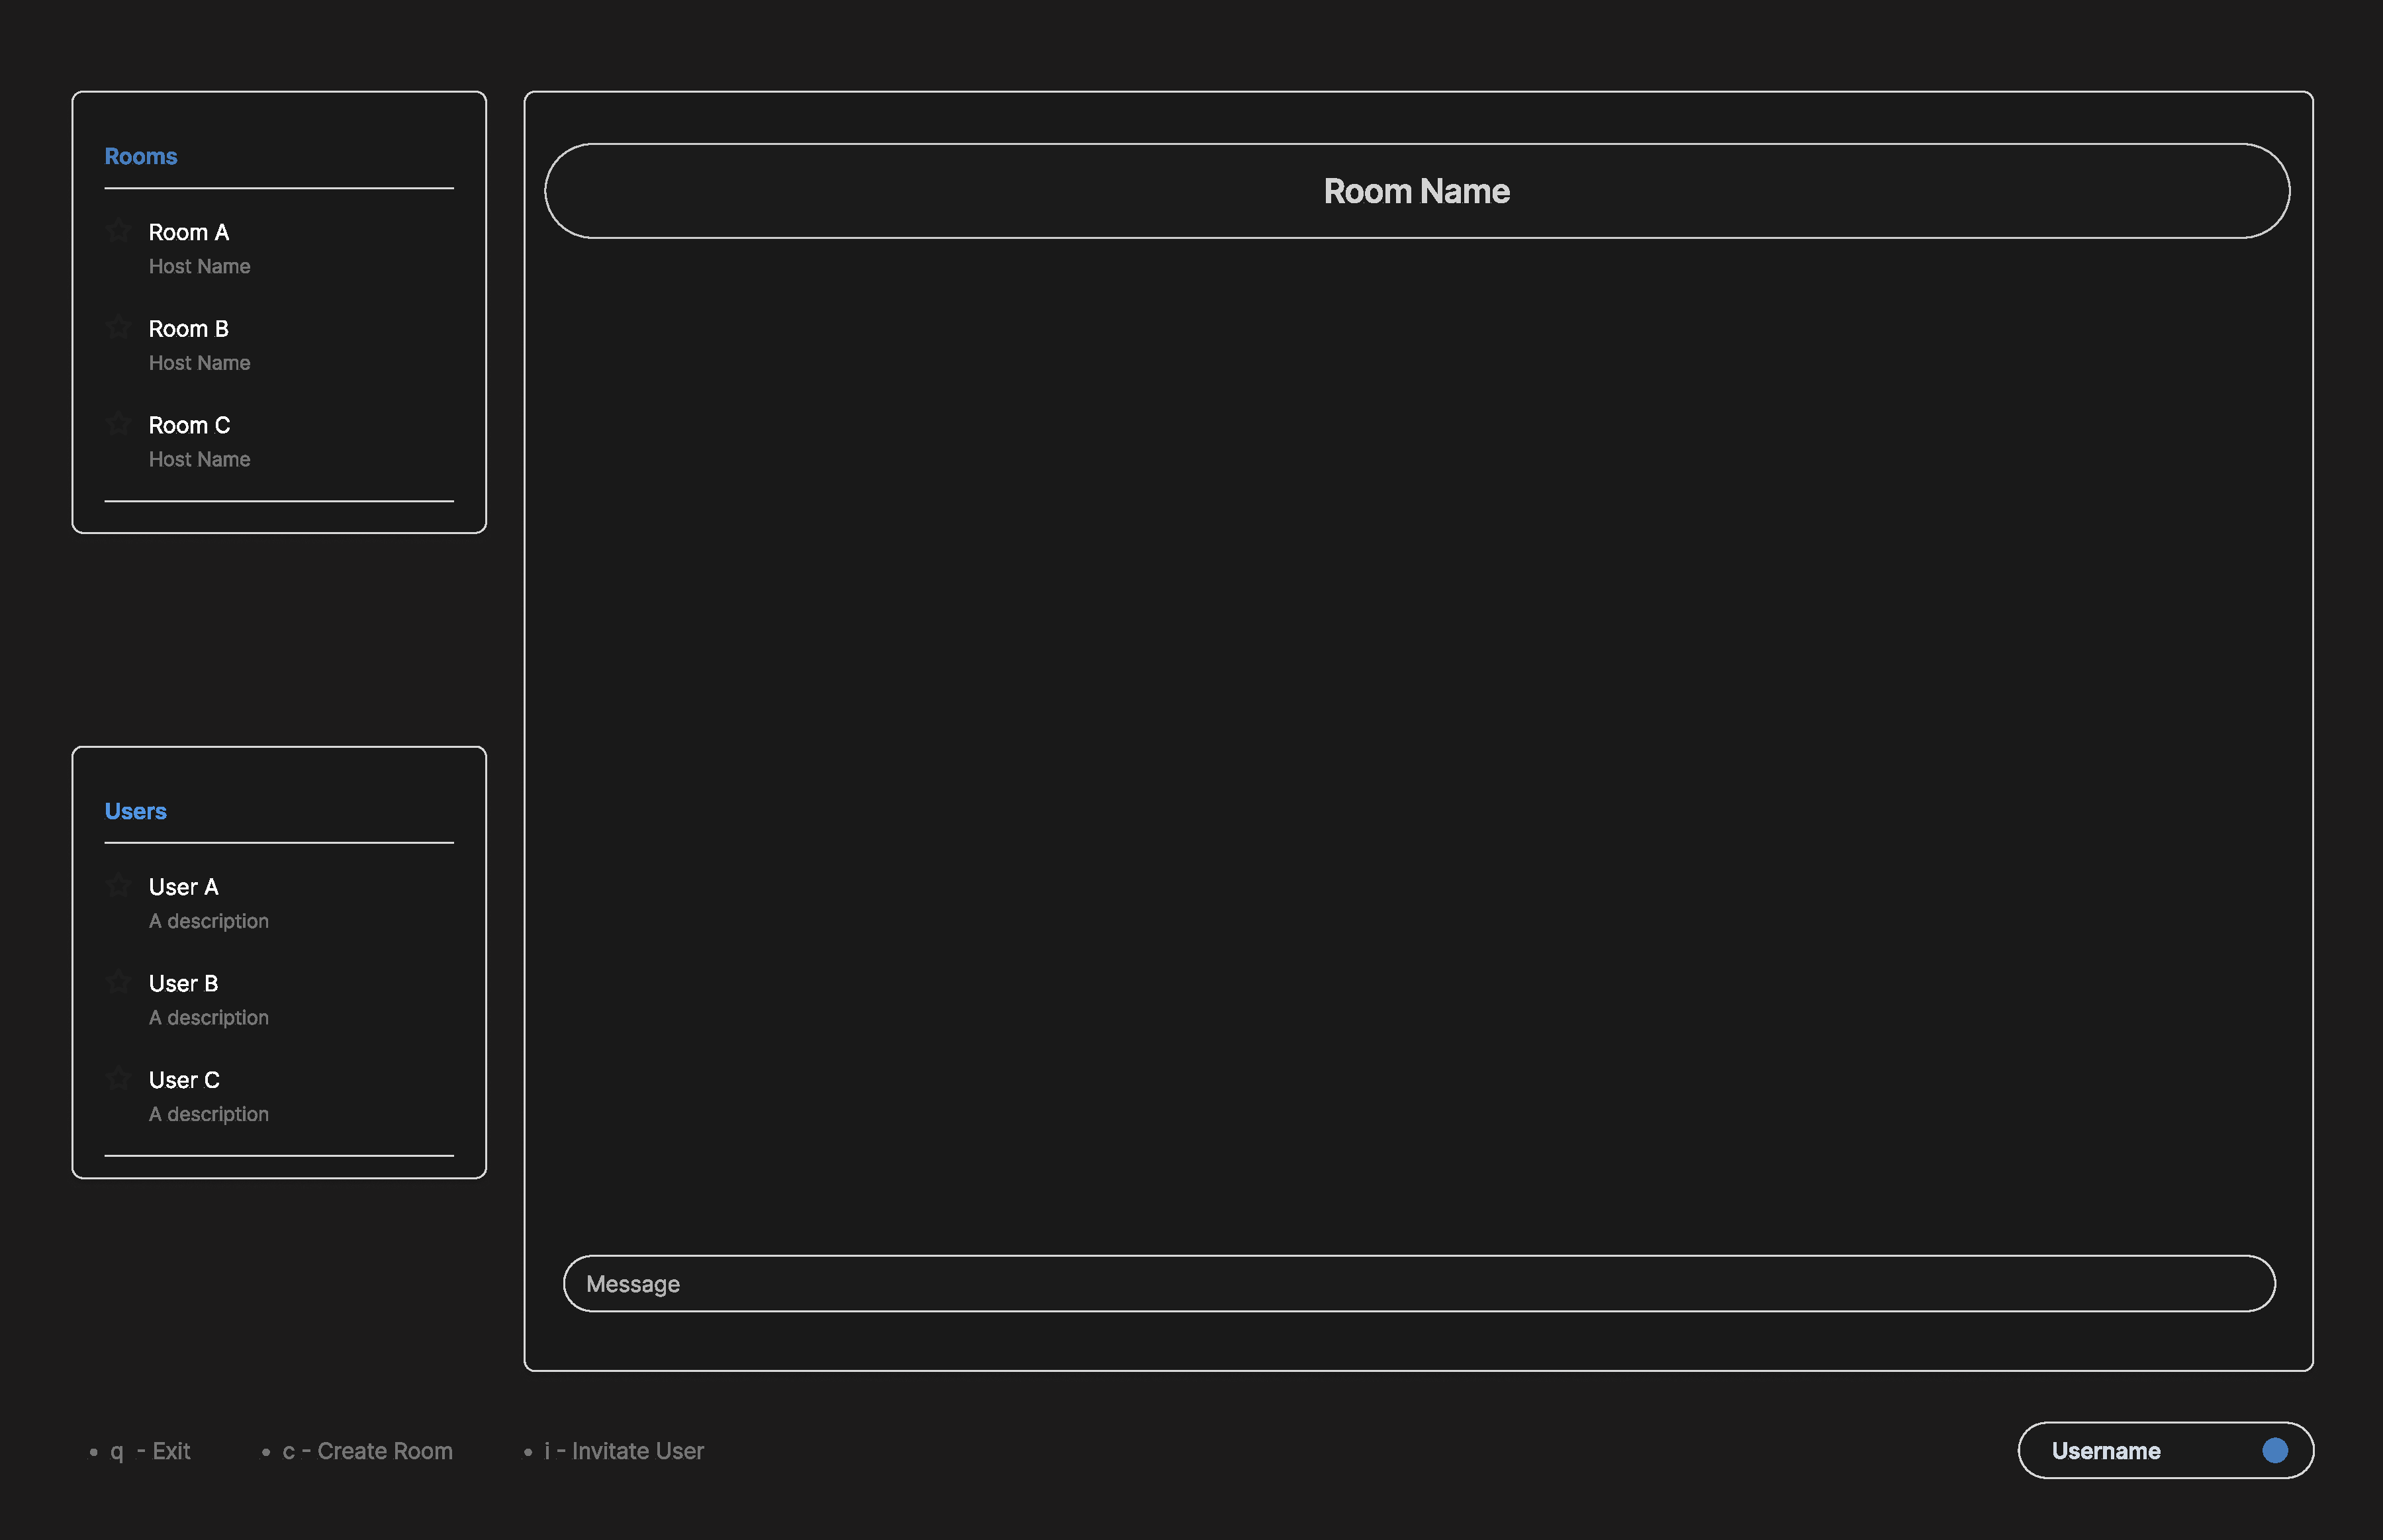
\includegraphics[width=0.8\textwidth]{landing.pdf}
    \caption{Mockup de la interfaz de terminal del cliente.}
    \label{fig:mockup-cliente}
\end{figure}

La vista principal se compone de cuatro paneles persistentes organizados en pantalla:

\begin{table}[h]
    \centering
    \begin{tabular}{lp{11cm}}
        \textbf{Panel} & \textbf{Descripción} \\
        \textbf{Panel de cuartos} & Permite visualizar las salas a las que pertenece el usuario. \\
        \textbf{Panel de usuarios} & Despliega la lista de usuarios conectados en el servidor. \\
        \textbf{Panel de chat} & Es el panel principal de la aplicación. Contiene un \textit{viewport} para el scroll y visualización de texto, y un \textit{textinput} para manejar el envío de mensajes. \\
        \textbf{Footer contextual} & Ubicado en la parte inferior de la pantalla, actualiza dinámicamente los atajos de teclado disponibles y muestra el estado actual del cliente. \\
    \end{tabular}
    \caption{Componentes de la vista principal del cliente.}
    \label{tab:paneles-cliente}
\end{table}

Además, para realizar la captura de datos y decisiones del cliente se opta por utilizar vistas \textbf{modales}. Es decir, interfaces superpuestas 
al contenido principal que bloquean temporalmente la interacción con el resto de la aplicación hasta que el usuario realiza una acción o la cierra. 

\begin{table}[h]
    \centering
    \begin{tabular}{lp{11cm}}
        \textbf{Modal} & \textbf{Descripción} \\
        \textbf{Input Modal} & Captura cadenas de texto del usuario. \\
        \textbf{List Modal} & Permite la selección simple o múltiple de los items mostrados por una lista. \\
        \textbf{Confirm Modal} & Permite ejecutar operaciones binarias excluyentes. \\
        \textbf{Notification Modal} & Despliega mensajes de notificación. \\
        \textbf{Wizard Modal} & Presenta flujos secuenciales de múltiples pasos con estado compartido. \\
    \end{tabular}
    \caption{Modales utilizados en el cliente.}
    \label{tab:modales-cliente}
\end{table}

El diseño de la interfaz de \textbf{Gabby} utiliza paneles genéricos embebidos en el \textbf{Modelo}
principal. De esta manera se desacoplan los tipos de datos de \textbf{dominio} de la lógica visual,
permitiendo, por ejemplo, reutilizar componentes entre distintos paneles. Esto se puede observar en el
diagrama de la figura \ref{fig:panels-uml} con el modelo de lista y los paneles tanto de usuarios como
de salas.

\begin{figure}[h]
    \centering
    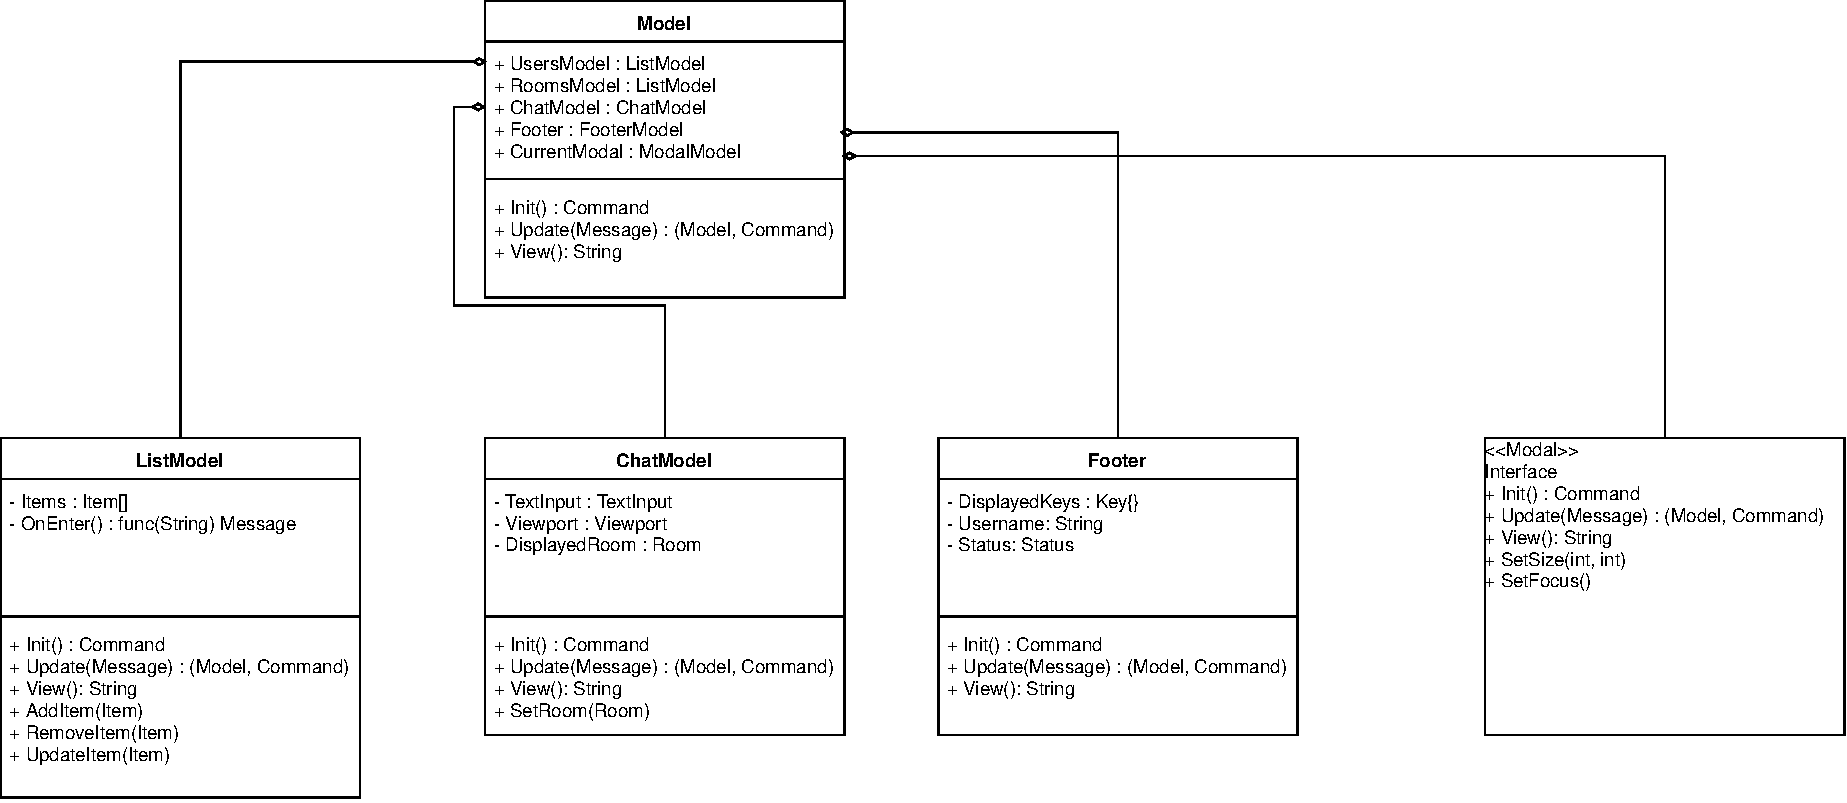
\includegraphics[width=1\textwidth]{panels.pdf}
    \caption{Diagrama UML de la organización de paneles.}
    \label{fig:panels-uml}
\end{figure}

Además, el diseño se simplifica gracias a los componentes prefabricados de \textbf{Bubbles}, la
biblioteca hermana de \textbf{Bubble Tea}. Específicamente, \textbf{Bubbles} ofrece tres componentes
esenciales para \textbf{Gabby}: \textbf{viewport} (permite el scroll del historial de mensajes), \textbf{textinput} 
(maneja la captura de texto) y \textbf{footer}, convirtiendo a algunos de los modelos principales en, básicamente, 
\textit{wrappers} sobre estos componentes.

La interacción de los modales con la vista principal depende de la implementación de la interfaz
\textbf{Modal}. El polimorfismo de modales permite abstraer su comportamiento común y simplificar la
visualización y el control de cada tipo de panel modal. Principalmente, nos permite modelar la interfaz
como una máquina de estados, donde la existencia de un \texttt{CurrentModal} activo determina el estado
de \textbf{captura}: mientras un modal esté presente, el modelo raíz le delega la totalidad de los
mensajes de entrada, secuestrando el control de la interfaz hasta que el modal se resuelve y \texttt{CurrentModal} vuelve a quedar vacío.

\begin{figure}[h]
    \centering
    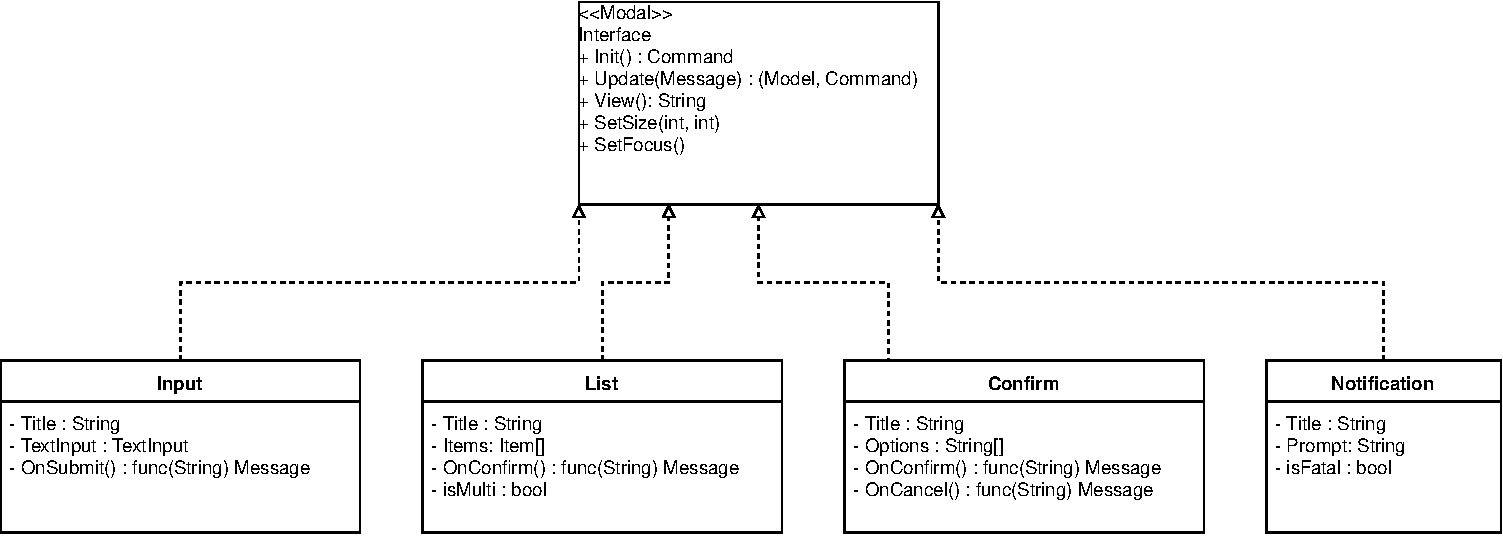
\includegraphics[width=1\textwidth]{modals.pdf}
    \caption{Diagrama UML de la organización de modales.}
    \label{fig:modals-uml} 
\end{figure}

\subsubsection*{Modelos de Dominio}

La presentación de la interfaz depende en gran medida de los datos mostrados. Es bastante intuitivo modelar los datos
básicos dado el contexto: \textbf{User} y \textbf{Room}. El usuario guarda un username y un estado.
La sala guarda un roomname, una lista de usuarios y un historial de mensajes (dado que el servidor no tiene persistencia).
Precisamente por eso, \textbf{Session} almacena en memoria el estado de un cliente, es decir su identidad,
sus salas disponibles, los usuarios conectados, las salas globales y los mensajes privados.

\subsubsection*{Capa de Red}

Cualquier aplicación de terminal realizada con \textbf{Bubble Tea} opera en un único hilo de
renderizado. Por lo tanto, intentar leer el socket TCP mediante el mismo hilo de ejecución provocaría
que la aplicación se bloqueara por completo. 

\textbf{Go} tiene un principio bastante interesante acerca de la comunicación asíncrona: \textit{``Do not 
communicate by sharing memory; instead, share memory by communicating''}. Esto se logra a través de canales 
que permiten para pasar referencias a datos entre goroutines.

De está manera podemos utilizar una goroutine independiente para leer los datos del socket, comunicar las lecturas
a un canal y utilizar los \textbf{cmd} de \textbf{Bubble Tea} para inyectar los \textbf{messages} en la función 
\textbf{Update} del Modelo raíz. Este flujo se puede observar de mejor manera en el diagrama \ref{fig:conn}.

\begin{figure}[h]
    \centering
    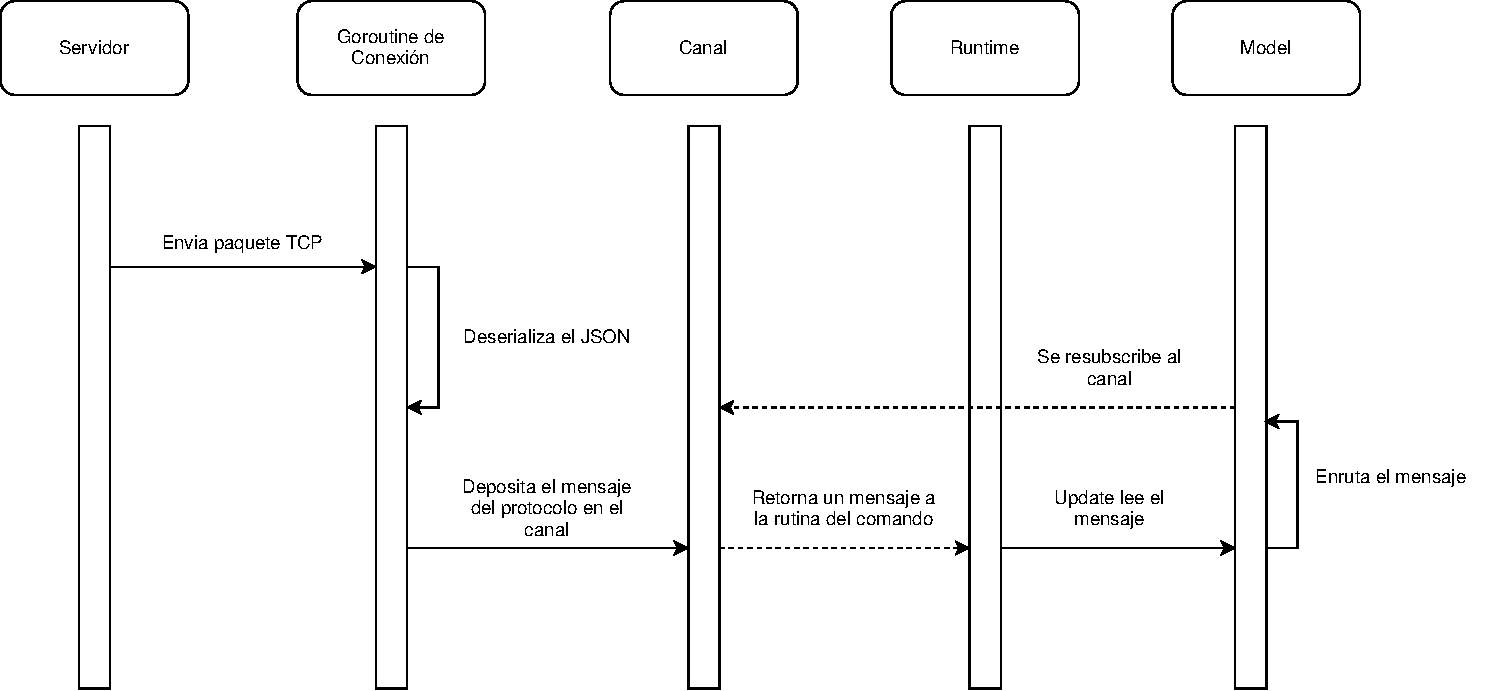
\includegraphics[width=0.8\textwidth]{conn.pdf}
    \caption{Diagrama de secuencia de la interacción por red.}
    \label{fig:conn} 
\end{figure}

\subsubsection*{Enrutamiento}

El método \textbf{Update} del modelo raíz centraliza el despacho de eventos clasificándolos en tres dominios principales.

\begin{description}[leftmargin=2.2cm, style=nextline, font=\bfseries]
    \item[Mensajes del Servidor] Representa los mensajes y respuestas entrantes del servidor.
    \item[Mensajes del Cliente] Representa los mensajes enviados por el cliente.
    \item[Mensajes Internos] Representa mensajes de cambio interno en la interfaz.
\end{description}

Cada uno de ellos cuenta con un \textbf{Router} que mapea cada tipo de mensaje a una función \textit{handler}.


\subsection*{Servidor}

\textbf{Fearless Concurrency} es el principio fundamental de la elección del lenguaje de programación
\textbf{Rust} para el desarrollo del servidor. Muchas de las implementaciones de seguridad de memoria
que incluye el lenguaje, mediante su sistema de \textit{ownership} y \textit{borrowing} permiten transformar 
errores en tiempo de ejecución a errores en tiempo de compilación. De esta manera, \textit{data races} y 
otros errores comunes en programación concurrente, que en otros lenguajes solo se manifiestan durante la ejecución,
son detectados por el compilador antes de que el programa siquiera se ejecute. Esto permite escribir código
concurrente con la confianza de que, si compila, está libre de una clase entera de errores que tradicionalmente son 
difíciles de depurar y reproducir.

El modelo de programación asíncrona de \textbf{Rust} presenta una particularidad importante:
tanto la sintaxis \texttt{async}/\texttt{await} como el trait \texttt{Future} están definidos
a nivel del lenguaje y su biblioteca estándar, pero se trata de implementaciones \textbf{lazy}
que no se ejecutan por sí solas, ya que \textbf{Rust} no incluye un entorno de ejecución asíncrono.
Para esto, utilizamos \textbf{Tokio}, el entorno de ejecución asíncrono más popular dentro de la 
comunidad de \textbf{Rust}. 

El entorno de ejecución de \textbf{Tokio} es bastante rápido debido a su arquitectura basada en un diseño
modular y de alto rendimiento enfocado en el I/O no bloqueante. Se basa principalmente en el patrón de diseño
\textbf{Reactor} que permite manejar múltiples \textbf{tasks} en un solo hilo de ejecución, con la ayuda de un 
\textbf{task scheduler}, un \textbf{I/O Driver} y \textbf{timers} que se comunican directamente con el sistema
operativo. 

\textbf{Tokio} también ofrece varias abstracciones de alto nivel y macros que permiten trabajar fácilmente la programación
asíncrona.

\subsubsection*{Arquitectura}

El estado de la aplicación se centraliza en una única estructura de estado global (\texttt{Hub})
que administra a todos los clientes, salas públicas y salas privadas activas en el servidor.
Internamente, el \texttt{Hub} almacena estas entidades en diccionarios (\texttt{HashMap}),
indexados por el nombre de usuario o de sala, lo que permite consultas en tiempo $O(1)$ amortizado.

\begin{figure}[h]
    \centering
    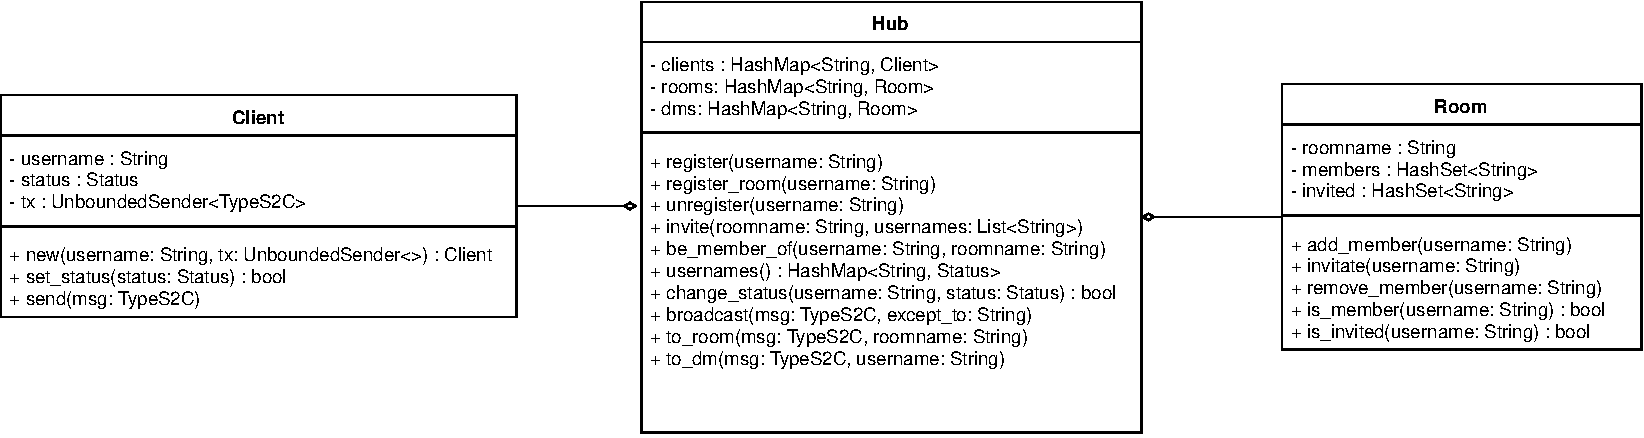
\includegraphics[width=1\textwidth]{hub.pdf}
    \caption{Diagrama UML del servidor.}
    \label{fig:hub} 
\end{figure}

Además, como puede observarse en el diagrama de la figura \ref{fig:hub}, el \texttt{Hub} funciona
como mediador entre los múltiples clientes conectados y es el encargado de ejecutar la mayoría de
las operaciones definidas en el protocolo. De esta manera, no existe comunicación directa entre
clientes (\textbf{P2P}), ya que toda interacción debe pasar necesariamente a través del \texttt{Hub}.

Las salas mantienen su propio estado internamente, utilizando conjuntos (\texttt{HashSet}) para
almacenar tanto a sus miembros como a sus invitados. De esta manera, se simplifica la lógica
encargada de enrutar mensajes y eventos hacia las salas correspondientes.

\subsection*{Conexiones}

Cada vez que entra un nuevo cliente al servidor, \textbf{Tokio} delega la conexión del socket a un \textbf{task}
independiente, que se encarga de manejar la comunicación con el usuario. El primer paso de la comunicación siempre
consiste en identificarse; si la tarea verifica la correctitud de la identificación, crea un \textbf{Client} y lo
registra en el \textbf{Hub}. 

En la figura \ref{fig:hub}, podemos notar que los \textbf{Client} no guardan una referencia del socket, si no que guardan
un canal MPSC (\textit{Multiple Producer, Single Consumer}). El canal permite desacoplar las tareas de I/O relacionadas al
socket, y permitir que cada conexión se gestione sola.

Después de la identificación, la \textbf{task} entra en un bucle que multiplexa dos fuentes de eventos
asíncronos mediante la macro \texttt{tokio::select!}:

\begin{enumerate}

    \item \textbf{Lectura del Socket}: Escucha los mensajes que llegan a través del socket TCP, deserializa el mensaje
        y lo transfiere al \textbf{enrutador} para ejecutar la acción correspondiente.

    \item \textbf{Lectura del Canal}: Escucha los mensajes entrantes al canal, extra el mensaje y lo transmite por el socket
        TCP hacia el cliente.

\end{enumerate}

Mediante este mecanismo, el runtime suspende la tarea hasta que alguno de los dos \textit{futures} esté
listo, procesando de inmediato el primer evento disponible.

\begin{figure}[h]
    \centering
    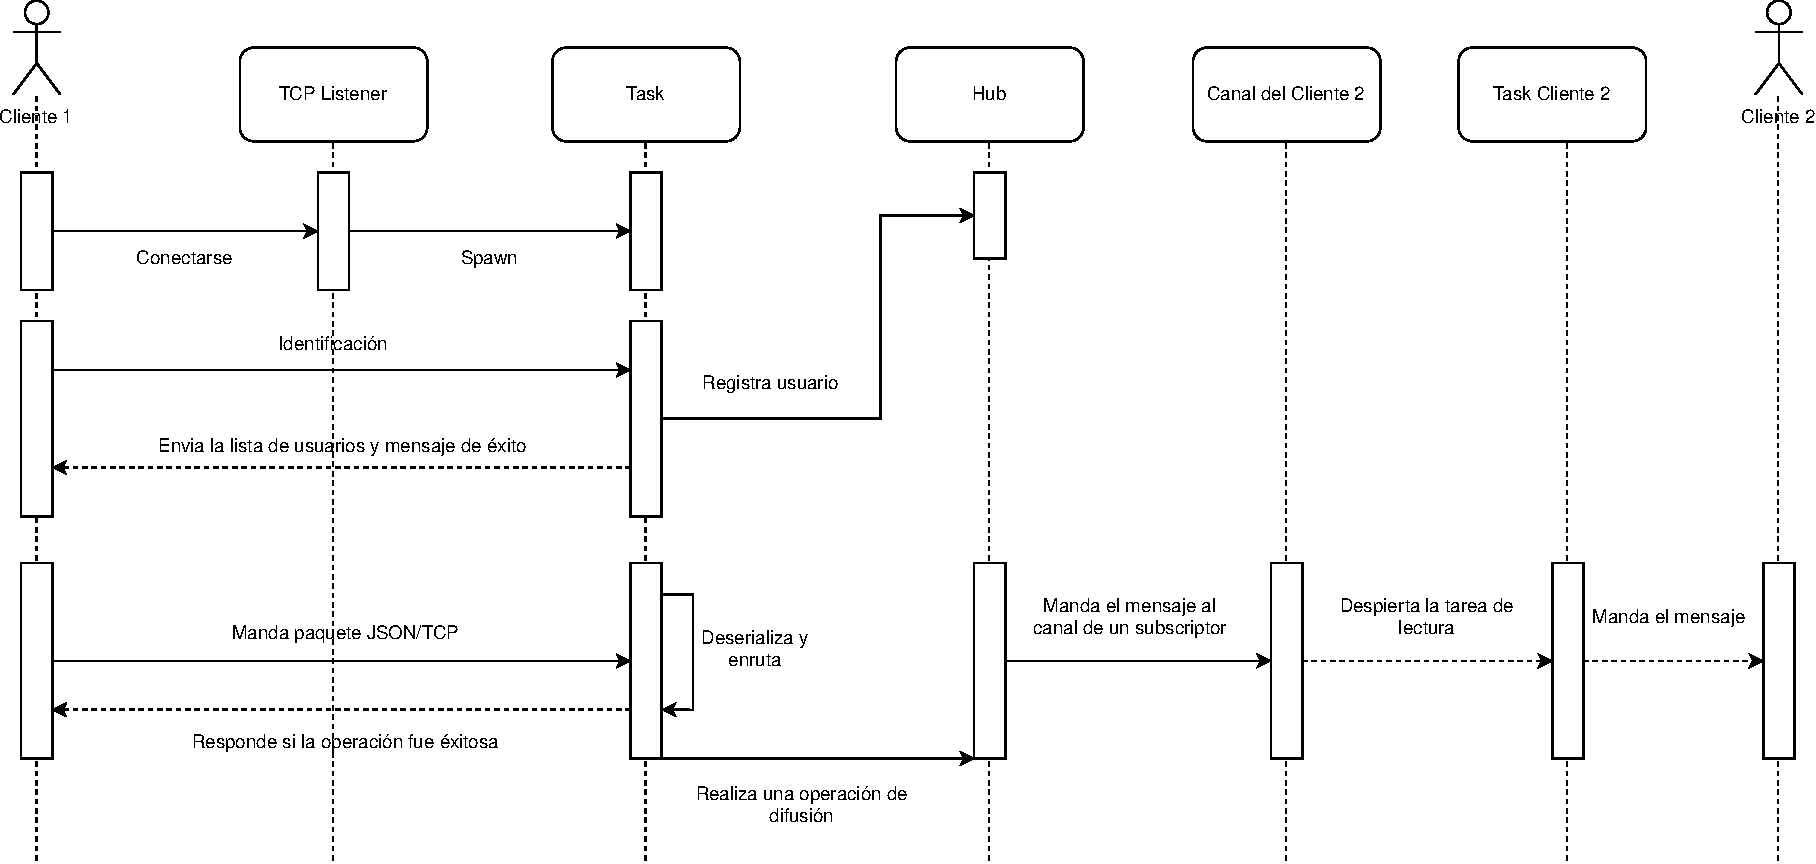
\includegraphics[width=1\textwidth]{server-flow.pdf}
    \caption{Diagrama de secuencia del servidor.}
    \label{fig:server-sequence} 
\end{figure}

Las \textbf{tasks} necesitan modificar concurrentemente el estado global de la sesión (\textbf{Hub}) 
para realizar la mayoría de las operaciones del protocolo. Una solución idiomática en \textbf{Rust} 
para este problema es la combinación \texttt{Arc$<$Mutex$<$Hub$>$$>$}. Por un lado, \texttt{Arc} (\textit{Atomically 
Reference Counted}) es un apuntador inteligente que permite compartir la propiedad de un mismo dato, 
en este caso la instancia global del \textbf{Hub}, entre múltiples tareas de forma segura. Por otro lado, 
\texttt{Mutex}, aunque cumple una función similar a un semáforo en la mayoría de los lenguajes, en 
\textbf{Rust} se comporta de manera distinta: en lugar de ser un mecanismo externo que protege el acceso 
a una variable, el \texttt{Mutex} envuelve directamente al dato, de modo que resulta imposible acceder a 
él o mutarlo sin antes adquirir el cerrojo.

\subsubsection*{Enrutamiento y Protocolo} 

\textbf{Rust} permite modelar información mediante \textbf{tipos de datos suma} a través de sus
enumeraciones. Un tipo suma representa un valor que solo puede adoptar una de varias formas posibles,
donde cada variante puede llevar asociados datos de tipos distintos entre sí. Los \textbf{tipos de datos suma}, 
ofrecen importantes ventajas de seguridad de tipos, en particular la posibilidad de realizar \textbf{pattern matching}
exhaustivo, es decir un manejo explícito de todos los casos con verificación del compilador.

El \textbf{protocolo} del servidor modela la comunicación mediante dos tipos suma: \textbf{ClientMessage}, que representa
los mensajes enviados del cliente al servidor, y \textbf{ServerMessage}, que representa los mensajes enviados del servidor
al cliente. Ambos tipos de dato, se serializan y deserializan con la biblioteca de \textbf{serde}, por medio del etiquetado 
interno.

Los mensajes \textbf{deserializados} válidos se delegan a una función \textbf{router}, la cual realiza internamente un
\textit{match} sobre el \textbf{ClientMessage}. El \textbf{pattern matching} permite mapear fácilmente cada variante a 
una función auxiliar \textbf{handler}, encargada de manejar la operación correspondiente, típicamente modificando el estado
global y difundiendo mensajes \textbf{ServerMessage} al resto de los clientes.
 \section{Implementación}

\subsection*{Estructura}

Dado el alcance del proyecto, la organización del repositorio se realizó mediante un \textbf{monorepo}. Lo anterior,
permite centralizar el código tanto del cliente, como del servidor, y orquestar tareas comúnes de desarrollo.

\dirtree{%
    .1 ./.
    .2 client/.
    .3 cmd/.
    .4 client/.
    .3 internal/.
    .4 domain/.
    .4 network/.
    .4 protocol/.
    .4 ui/.
    .5 messages/.
    .5 panels/.
    .5 styles/.
    .2 docs/.
    .3 mockups/.
    .3 report/.
    .4 figures/.
    .4 sections/.
    .3 tapes/.
    .2 server/.
    .3 src/.
    .4 protocol/.
    .2 stress/.
}

Por un lado, el \textbf{Client} se organiza siguiendo la
\href{https://github.com/golang-standards/project-layout/blob/master/README_es.md}{Standard Go
Project Layout}, la organización estándar de proyectos en \textbf{Go}. Utiliza \textbf{cmd} para
el punto de entrada del cliente e \textbf{internal} para organizar el código interno, relacionado
tanto con la lógica de negocio como con la vista de usuario.

Por otro lado, el \textbf{servidor} se organiza de una manera más simple, en un único
\textbf{crate} que centraliza el comportamiento general de la aplicación. Únicamente el protocolo
se separa en su propio módulo.

\subsection*{Dependencias}

Las dependencias del desarrollo se listan en la la tabla \ref*{tab:requisitos}.

\begin{table}[h]
    \centering
    \begin{tabular}{ll}
        \textbf{Componente} & \textbf{Versión} \\ \hline
        \textbf{Go} & 1.26.6 \\
        \textbf{Bubble Tea} & 1.3.10 \\
        \textbf{Lipgloss} & 1.1.0 \\
        \textbf{Bubbles} & 1.0.0 \\
        \textbf{Rust} & 1.97.1 \\
        \textbf{Tokio} & 1.53.1 \\
        \textbf{Serde} & 1.0.229 \\
        \textbf{Serde JSON} & 1.0.151 \\
        \textbf{Just} & 1.57.0 \\
        \textbf{Prek} & 0.5.0 \\
        \textbf{k6} & 2.3.0 \\
        \textbf{xk6-tcp} & main \\
    \end{tabular}
    \caption{Requisitos y dependencias del proyecto.}
    \label{tab:requisitos}
\end{table}

\subsection*{Flujo de Trabajo}

Para unificar los sistemas de compilación, ejecución de pruebas unitarias, documentación y ejecución de ambos
programas, se utilizó \textbf{Just}. Por ejemplo, el siguiente comando realiza el build tanto del cliente como del servidor.

\begin{lstlisting}[language=bash]
    just build
\end{lstlisting}

Además, para mantener una consistencia de código se utiliza \textbf{Prek} para realizar un formateo del código,
tanto de \textbf{Rust} como de \textbf{Go}, antes de cada commit.

La mayoría del flujo inicial se basó en el flujo de trabajo \textit{code a little, test a little}. Las pruebas unitarias
se ejecutan en \textbf{workflows} de \textbf{integración continua} durante cada push.

\subsection*{Servidor}

Observemos como se translada el modelo del servidor al código. 

\subsubsection*{Multiplexado}

La macro \texttt{tokio::select!} permite ejecutar concurrentemente varias expresiones en la misma \textbf{task}. De está manera, 
ambas fuentes de eventos alternan su ejecución dependiendo del cumplimiento de las ramas.

\begin{lstlisting}[language=Rust]
tokio::select! {
    // 1. Lectura del socket TCP
    result = reader.read_line(&mut line) => {
        match result {
            Ok(0) => break, // EOF
            Ok(_) => {
                if let Ok(msg) = serializer::deserialize(&line) {
                    if let Err(err) = route_msg(msg, &_username, &hub, &mut writer).await {
                        send_msg(&mut writer, new_response(TypeC2S::Invalid, err, None)).await;
                        break;
                    }
                }
            }
            Err(_) => break,
        }
    }

    // 2. Recepcion de mensajes salientes desde el canal MPSC
    Some(msg) = rx.recv() => {
        send_msg(&mut writer, msg).await;
    }

    else => break,
}
\end{lstlisting}

\subsubsection*{Enrutamiento}

La función de enrutamiento implementa el patrón de descrito en la \autoref{sec:analisis-diseno}: recibe un 
\texttt{ClientMessage} ya deserializado y, mediante un \texttt{match} exhaustivo sobre sus variantes, delega 
la operación correspondiente a una función \textit{handler} específica.

\begin{lstlisting}[language=Rust]
async fn route_msg<W>(
    msg: ClientMessage,
    username: &str,
    hub: &Arc<Mutex<Hub>>,
    writer: &mut W,
) -> Result<(), MessageResult>
where
    W: AsyncWrite + Unpin,
{
    match msg {
        ClientMessage::Users => handle_users_list(hub, writer).await,
        ClientMessage::Status { status } => handle_status(username, status, hub).await,
        ClientMessage::PublicText { text } => handle_public_text(username, &text, hub).await,
        ClientMessage::NewRoom { roomname } => {
            handle_create_room(username, &roomname, hub, writer).await?;
        }
        ...
    }
}
\end{lstlisting}

\subsubsection*{Estado Compartido}

La mayoría de funciones \texttt{handler} recibe un \texttt{\&Arc$<$Mutex$<$Hub$>$$>$}. Está es una manera popular en la comunidad
de \textbf{Rust} para implementar el \textbf{estado compartido por exclusión mutua} para realizar modificaciones en un estado global.
Sin embargo, la cautela al abrir el bloqueo tiene que realizarse minuciosamente y abarcando la menor cantidad de 
operaciones.

Por ejemplo, apoyanse ampliamente de \textit{scopes} resulta indispensable. 

\begin{lstlisting}[language=Rust]
let result = {
    let hub = hub.lock().unwrap();
    hub.send_to(&msg, sender, receiver)
    // El hub se libera al salir de este scope
};

match result {
    Ok(_) => {}
    Err(e) => {
        send_msg(
            writer,
            new_response(TypeC2S::Text, e, Some(receiver.to_string())),
        )
        .await;
    }
}
\end{lstlisting}

\subsection*{Cliente}

\subsubsection*{Concurrencia en el Cliente}

Mantener sincronizada la interfaz de usuario con el estado global del servidor sin bloquear el hilo de
renderizado es una tarea indispensable para aplicaciones con interfaces visuales. Por está razón, la 
concurrencia resulta igual de necesaria en la capa del \textbf{cliente} que en \textbf{servidor}; no quieres
ofrecer una experiencia de usuario lenta y poco responsiva.

La conexión se encuentra desacoplada de la interfaz y corre en una \textbf{goroutine} secundaria. Por cada
línea que lee del buffer, si no está malformada, se deserializa y se envía a un canal.

\begin{lstlisting}[language=Go]
// Listen escucha los mensajes del servidor al cliente y los manda a traves de un canal
func (manager *ConnectionManager) Listen() {
	for {
		line, err := manager.reader.ReadString('\n')
		if err != nil {
			log.Printf("Connection closed: %v", err)
			return
		}

		msg, err := protocol.Deserialize(line)

		if err != nil {
			log.Printf("Invalid message: %s", line)
			continue
		}

		manager.incoming <- msg
	}
}
\end{lstlisting}

El modelo principal espera mensajes de ese canal. Cuando recibe alguno, retorna un comando con el mensaje
ya deserializado.

\begin{lstlisting}[language=Go]
func (m Model) waitForServerMsg() tea.Cmd {
    return func() tea.Msg {
        return <-m.conn.Messages()
    }
}
\end{lstlisting}

El mensaje es capturado por \textbf{Update} y delegado al \textit{router} de mensajes del servidor. Una vez
procesado, el modelo se resubscribe al canal en espera de más mensajes.

\begin{lstlisting}[language=Go]
func (m Model) Update(msg tea.Msg) (tea.Model, tea.Cmd) {
	switch msg := msg.(type) {

	case protocol.ClientMessage:
		return m, m.routeClientMessage(msg)

	case protocol.ServerMessage:
		cmd := m.routeServerMessage(msg)
        // Se resuscribe al canal
		return m, tea.Batch(cmd, m.waitForServerMsg())

	return m, nil
}
\end{lstlisting}

\subsection*{Modales}

Los modales utilizados en la interfaz por terminal implementan la interfaz descrita en la
\autoref{fig:modals-uml}. Cada tipo de modal (\texttt{Input}, \texttt{List}, \texttt{Confirm},
\texttt{Notification}) satisface esta interfaz, lo que permite al modelo raíz tratarlos de manera
uniforme.

El modelo raíz contiene un campo \texttt{activeModal} que implementa la máquina de estados descrita
en el diseño: mientras este campo esté activo, se le delega la totalidad del flujo de entrada hasta
resolverse.

\begin{lstlisting}[language=Go]
type Modal interface {
    InputCapturer
    Init() tea.Cmd
    Update(msg tea.Msg) (Modal, tea.Cmd)
    View() string
    Focus() tea.Cmd
    SetSize(width, height int)
}
\end{lstlisting}

Por ejemplo, un evento puede invocar la creación de un modal y establecerlo en la vista principal.

\begin{lstlisting}[language=Go]
case "c":
    return m.openModal(panels.NewInputModal("Create Room", "Roomname", 16, func(value string) tea.Msg {
        room, _ := protocol.NewRoomMessage(value)
        return room
    }, true))
\end{lstlisting}

La función \texttt{openModal} realiza la transición de estado \textit{sin modal} a \textit{modal
activo}, y espera a que el modal se resuelva en algún momento posterior.

\begin{lstlisting}[language=Go]
func (m *Model) openModal(modal panels.Modal) tea.Cmd {
    modal.SetSize(m.width, max(0, m.heigth-3))
    m.chatModel.Blur()
    cmd := modal.Focus()
    m.activeModal = modal
    // Inicializa el modal
    return tea.Batch(cmd, modal.Init())
}
\end{lstlisting}

Cuando el servidor responde exitosamente a la operación solicitada por el modal, el enrutador de mensajes 
del servidor resuelve el flujo: cierra el modal activo
y actualiza el estado local con la nueva información.

\begin{lstlisting}[language=Go]
if msg.Result == protocol.SUCCESS {
    m.closeModal()

    room := m.session.AddRoom(domain.RoomChannel, msg.Extra)
    m.roomsModel.AddItem(NewRoomItem(room))
}
\end{lstlisting}

Finalmente, \texttt{closeModal} realiza la transición inversa, devolviendo la interfaz al estado sin
captura.

\begin{lstlisting}[language=Go]
func (m *Model) closeModal() {
    m.activeModal = nil
    m.syncFocus()
}
\end{lstlisting}

\subsection*{Resultados}

Agregado a las pruebas unitarias, se crearon pruebas de éstres mediante una extensión de \textbf{K6} personalizada
para TCP, \textbf{xk6-tcp}. Las pruebas simulan un flujo concurrente de alta carga: 

\begin{enumerate}
    \item Conecta \textbf{3000} usuarios distribuidos en varias etapas.
    \item Cada usuario envía 5 mensajes públicos y espera 10 segundos.
    \item El usuario se desconecta.
\end{enumerate}

Los resultados obtenidos, se muestran en la siguiente tabla \ref{tab:estres}.

\begin{table}[htbp]
    \centering
    \small
    \begin{tabular}{lrr}
        \hline
        \textbf{Métrica} & \textbf{Total} & \textbf{Promedio} \\ \hline
        Pico de usuarios concurrentes & 3,000 & -- \\
        Conexiones TCP totales & 17,608 & 143.14 conn/s \\
        Errores de conexión & 1 & -- \\
        Escrituras TCP & 122,030 & 992.00 op/s \\
        Lecturas TCP & 2,582,224 & 20,991.38 op/s \\
        Datos enviados por clientes & 7.1 MB & 58 kB/s \\
        Datos distribuidos por servidor & 583 MB & 4.7 MB/s \\
        \hline
    \end{tabular}
    \caption{Resultados de la prueba de estrés TCP.}
    \label{tab:estres}
\end{table}
 \section{Conclusiones}

Se logró implementar un sistema de chat multicliente basado en la arquitectura cliente-servidor, cubriendo
por completo el protocolo establecido en clase, además de incorporar una interfaz de usuario por terminal.

El servidor se desempeñó de manera bastante decente incluso bajo una carga considerable. Aunque esperaba
que el sistema colapsara con un número mucho menor de usuarios concurrentes, los resultados muestran que soportó
3,000 usuarios simultáneos con una tasa de error prácticamente nula, al menos en el escenario simulado.

Sin embargo, el proceso de desarrollo estuvo lleno de altibajos y de una carga de nuevos conocimientos
abismal. En retrospectiva, creo haber tomado algunas decisiones técnicas sobreestimando mi capacidad de
aprendizaje y el tiempo disponible. Por ejemplo, desarrollar el proyecto en dos lenguajes con los que 
tenía muy poca experiencia previa, o dedicar una cantidad considerable de tiempo a módulos no 
estrictamente necesarios, como el diseño detallado de la interfaz de terminal. 

Precisamente, el tener que aprender tantos conceptos y tecnologías nuevas a la vez limitó el tiempo 
disponible para el modelado inicial, lo cual me llevó a tomar decisiones subóptimas para resolver ciertos
problemas, mismas que terminé pagando con refactorizaciones.

Ahora que comprendo mejor las tecnologías con las que trabajé, espero poder modelar y anticipar mejor los próximos 
proyectos. En particular, pretendo delimitar el alcance desde el inicio y administrar mejor mis módulos de
trabajo, para no invertir tanto tiempo decidiendo en qué trabajar cada día.

\end{document}